A topologia sempre foi vista como uma área de abstração da matemática, sem
espaço para aplicações. Ela é usada para o estudo de diversos espaços
em sua forma abstrata, auxiliando matemáticos em diversas demonstrações
de teoremas e dando uma base fundamental para grande parte da teoria matemática
usada no dia a dia~\cite{Poincare1895}.

Certas propriedades dos espaços topológicos são estudadas através da
topologia algébrica, dando algumas informações, como o número de componentes
conexas por caminhos de um espaço e buracos. A princípio esta é uma área altamente
abstrata da matemática,  nos últimos anos esta visão foi mudando,
com o desenvolvimento da Homologia Persistente e Análise Topológica de Dados.

Um conjunto de dados, geralmente um subconjunto finito de algum espaço métrico,
pode ser estudado através da homologia persistente e assim obtemos informações
topológicas do objeto em estudo.

O pipeline da análise topológica de dados pode ser divido nos seguintes passos:
\begin{enumerate}
  \item A entrada do algoritmo pode ser um conjunto de pontos ou alguma matriz
  de distância/similaridade do conjunto de dados.
  \item A construção de um objeto combinatorial em cima do conjunto de dados ou
  da matriz de distância. Geralmente uma filtração ou um complexo simplicial.
  \item A partir da filtração ou do complexo simplicial é possível extrair informações
  topológicas e geométricas do conjunto de dados, por exemplo o número de
  componentes conexas, como um algoritmo de Clustering.
  \item Por fim a interpretação dos dados obtidos e possível pós processamento
  para a utilização em outros algoritmos, como os de classificação ou regressão.
\end{enumerate}

Neste capítulo descrevemos de forma ingênua a homologia persistente, começando com
filtrações, passando pelos espaços vetoriais associados
aos complexos simpliciais e chegando ao algoritmo de homologia persistente.
Mostraremos também como interpretar os resultados obtidos.
A \autoref{fig:pipeline_hp} mostra os passos para utilizar esta ferramenta em um conjunto de dados.

\begin{figure}
  \centering
  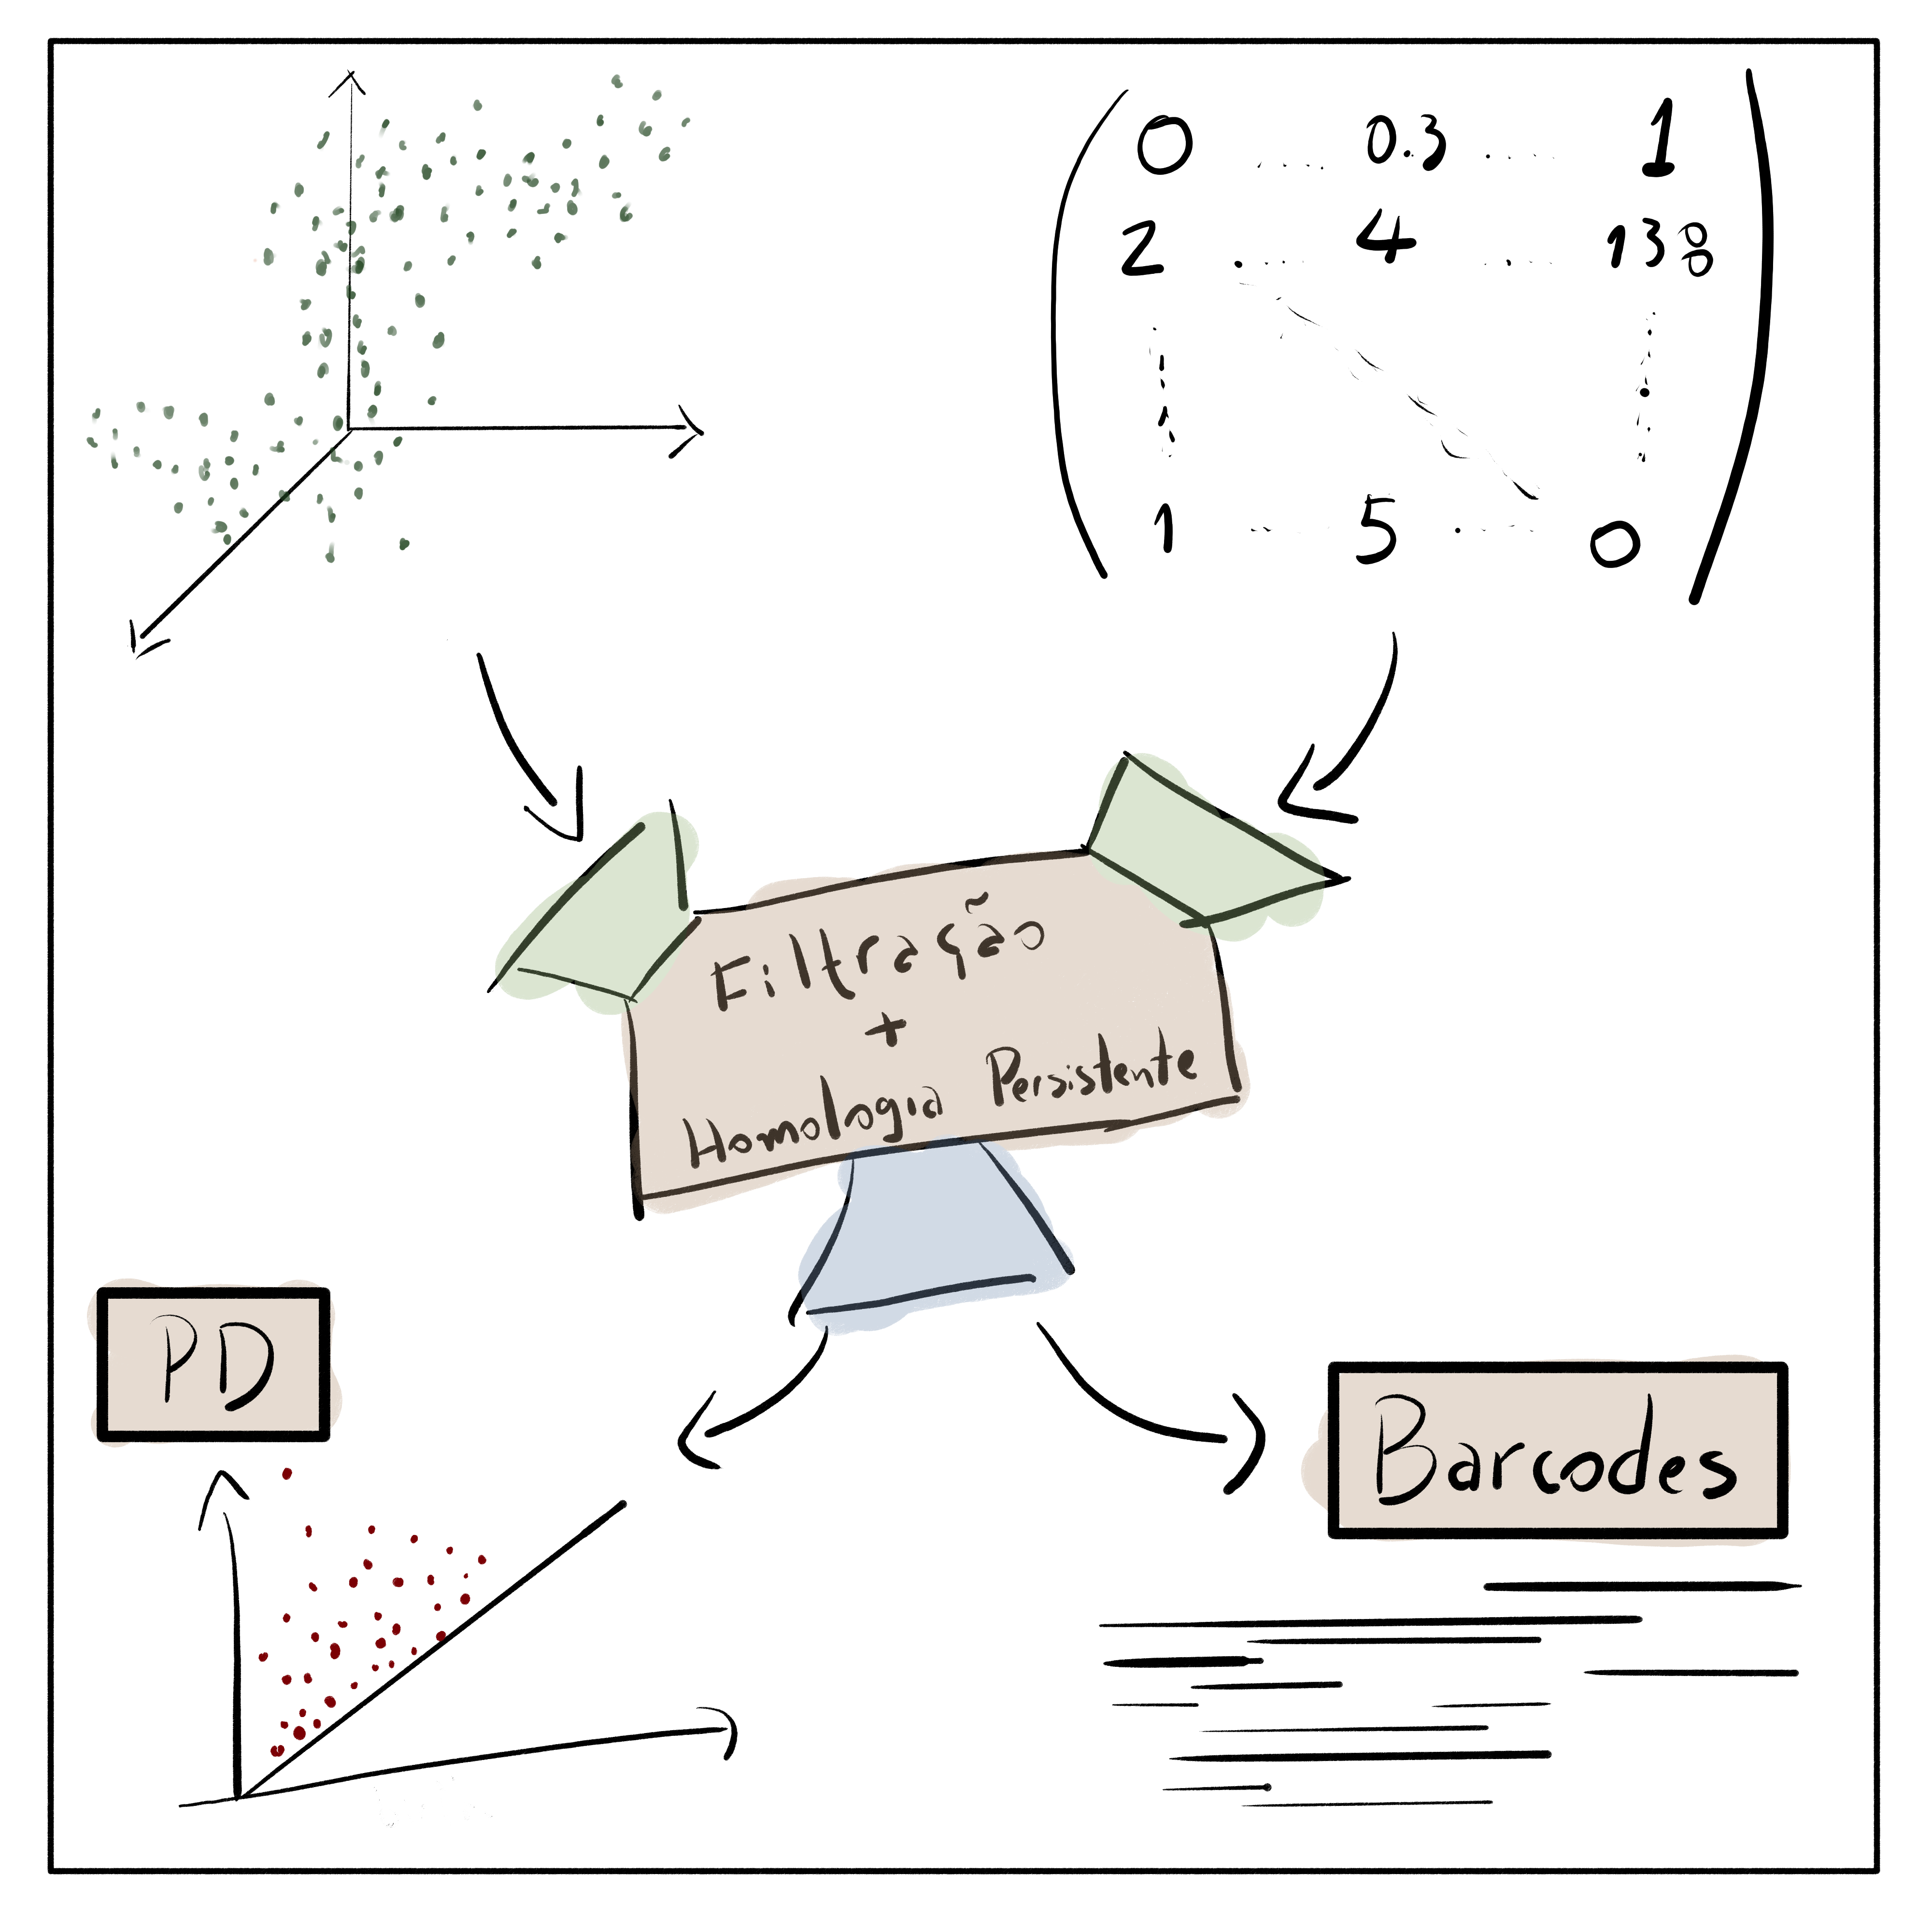
\includegraphics[width=0.7\textwidth]{images/pipeline_hp.png}
  \caption{Representação do pipeline para a utilização da homologia persistente
          com um conjunto de dados.}
  \label{fig:pipeline_hp}
  \fautor
\end{figure}


\section{Filtrações}
A filtração de um conjunto de dados é o primeiro passo na nossa sequência apresentada
na \autoref{fig:pipeline_hp}.
Dado um conjunto de dados precisamos construir um objeto combinatorial de forma
que possa ser analisado do ponto de vista da topologia assim como computacionalmente.
A filtração é este objeto que captura as mudanças do conjunto dada uma escala.

Algumas definições se fazem necessárias para entendermos o que é a filtração
e qual o seu papel na análise topológica de dados. Começamos definindo um simplexo,
primeiro objeto combinatorial que é a base da filtração.

\begin{defi}
  Sejam $v_0, v_1, \dots, v_k \in \mathbb{R}^n$ linearmente afins, ou seja $\Set{v_1 - v_0, \dots, v_k - v_0}$
  é um conjunto linearmente independente. O $k$-simplexo definido pelos pontos acima,
  chamados de vértices, é a envoltória convexa, definida na abaixo.
  \begin{equation}
    \label{eq:envconv}
    \Set{\sum_{i=0}^k \lambda_i v_i \ | \ \sum_{i=0}^k \lambda_i = 1 \text{ e }
          \lambda_i \ge 0, \ \forall i}.
  \end{equation}
  Denotamos o $k$-simplexo por $\langle v_0, \dots, v_k \rangle$.
\end{defi}

Note que para $k = 0$, temos um único vértice. Para $k=1$, temos uma reta, já
para $k=2$ temos um triângulo preenchido. E no caso $k=3$, um tetraedro. Os
simplexos podem ser vistos na~\autoref{fig:ksimpl}. Além disso, dizemos que a dimensão
do $k$-simplexo é $k$. A envoltória convexa de qualquer subconjunto dos vértices
de um simplexo $\sigma$ é chamado de face de $\sigma$.

\begin{figure}
  \centering
  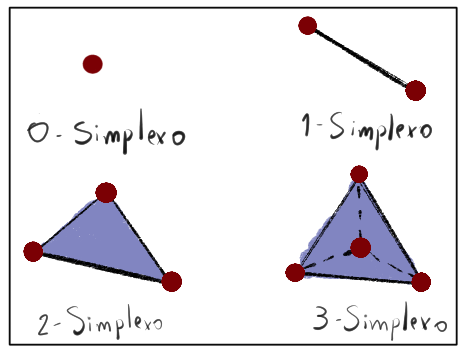
\includegraphics[width=0.7\textwidth]{images/ksimpl.png}
  \caption{Exemplos de $k$-simplexos para $k \in \Set{0,1,2,3}$.}
  \label{fig:ksimpl}
  \fautor
\end{figure}

Tendo definido os $k$-simplexos, podemos definir o complexo simplicial.
\begin{defi}
    Um complexo simplicial $K$ é uma coleção de simplexos satisfazendo as seguintes
    relações:
    \begin{itemize}
      \item Dado $\sigma \in K$, temos que para toda face $\tau \subset \sigma$
            vale $\tau \in K$.
      \item A interseção de dois simplexos é face de ambos os simplexos, em outras palavras,
      $\sigma, \tau \in K$ implica que $\sigma \cap \tau \subset \sigma$ e
      $\sigma \cap \tau \subset \tau$.
    \end{itemize}
\end{defi}
Nessa definição utilizamos o símbolo $\subset$ para indicar que uma face.
Usaremos esse símbolo com essa denotação quando falarmos sobre simplexos e
faces. A segunda condição é necessária para evitar casos patológicos como
mostrado na \autoref{fig:simp_path}. Dizemos que a dimensão do complexo
simplicial $K$ é a maior dimensão dentre os simplexos em $K$. Podemos definir
agora a filtração de um complexo simplicial.
\begin{figure}
  \centering
  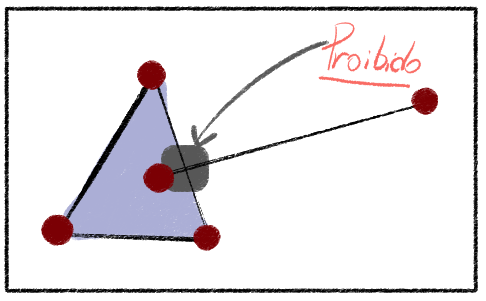
\includegraphics[width=0.7\textwidth]{images/simp_path.png}
  \caption{Exemplo em que a interseção de dois simplexos não é um simplexo.}
  \label{fig:simp_path}
  \fautor
\end{figure}
\begin{defi}
  Seja $K$ um complexo simplicial. Definimos uma filtração de $K$ sendo uma
  sequência de subconjuntos $K_i \subset K$, com $i \in \{ 1, \dots, n \}$,
  de tal forma que $K_i$ é um complexo simplicial para todo $i$ e vale que
  \begin{equation*}
    K_1 \subset \dots \subset K_{n-1} \subset K_n = K.
  \end{equation*}
\end{defi}
Na~\autoref{fig:filtracao_exemplo} temos um exemplo de filtração para um complexo
simplicial.

\begin{figure}[hbt]
  \centering
  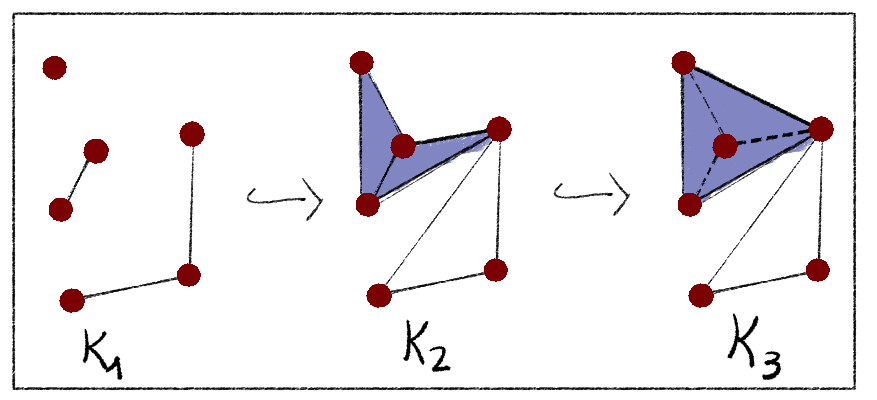
\includegraphics[width=0.7\textwidth]{images/filtracao_exemplo.png}
  \caption{Exemplo de filtração para um complexo simplicial $K$.}
  \label{fig:filtracao_exemplo}
  \fautor
\end{figure}


\subsection{Complexo de \v{C}ech}
Para construir complexos simpliciais a partir dos dados, precisamos abstrair
a noção de um simplexo simplicial. Na definição dada anteriormente, temos uma
representação geométrica do que é um simplexo, mas podemos abstrair tal noção
dando origem aos \textit{complexos simpliciais abstratos}. As definições para
os complexos definidos nesta seção e nas próximas foram retiradas de~\cite{edelsbrunner2010computational}.
\begin{defi}
  Seja $X$ um conjunto finito com pontos quaisquer. Seja $F$ um conjunto de
  subconjuntos não-vazios de $X$. Dizemos que $F$ é um complexo simplicial abstrato de
  $X$ se a seguinte condição é satisfeita.
  \begin{itemize}
    \item Se para todo $\sigma \in F$, temos que para todo subconjunto
          $\sigma' \subset \sigma$ está em $F$ também.
  \end{itemize}
  Cada elemento $\sigma \in F$ é chamado de simplexo. Denotamos um $k$-simplexo $\sigma$ por $\langle x_{i_0}, \dots, x_{i_k} \rangle$, onde $x_{i_j}$ são elementos de $X$.
\end{defi}

\begin{ex}
  Seja $X=\Set{a,b,c}$ e considere $F=\Set{\lp a \rp, \lp b \rp, \lp c \rp,
  \lp a,b \rp, \lp a,c \rp, \lp b,c \rp}$. Precisamos mostrar que F é um complexo
  simplicial abstrato. Seja $\sigma=\Set{a,c}$. Note que seus subconjuntos são
  $\Set{a}$ e $\Set{c}$, além disso ambos pertencem a $F$. De forma análoga, mostramos
  que para qualquer outro simplexo, suas faces (subconjuntos) estão em $F$.
\end{ex}
Podemos realizar os complexos simpliciais abstratos geometricamente, ou seja,
apesar de trabalharmos com conjuntos de elementos quaiser, podemos incluir
esses complexos em algum $\mathbb{R}^n$ e assim visualiza-los. Para obtermos
o complexo simplicial \textit{geométrico}, associamos a cada simplexo abstrato $\sigma$
um simplexo geométrico. Por exemplo, se adotarmos o complexo simplicial abstrato
$F$ acima mostrado, teriamos que sua realização geométrica seria um triângulo
sem preenchimento, como é mostrado na~\autoref{fig:abs_real}.

\begin{figure}
  \centering
  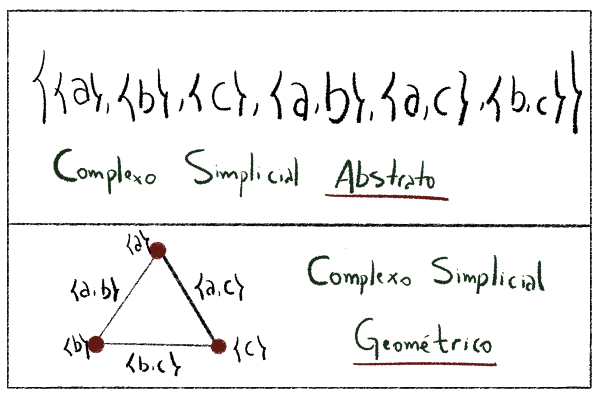
\includegraphics[width=0.7\textwidth]{images/abs_real.png}
  \caption{Exemplo de um complexo simplicial abstrato e sua realização geométrica}
  \label{fig:abs_real}
  \fautor
\end{figure}
Observe que se o nosso conjunto $X$ for um subconjunto finito de $\mathbb{R}^d$,
podemos ter simplexos de dimensão maiores do que $d$, ou seja, não podem ser
realizados (ou visualizados) em $\mathbb{R}^d$ necessariamente. Um exemplo dessa
situação pode ser visto no complexo simplicial final da \autoref{fig:filtracao_exemplo},
considerando que os pontos vermelhos são a realização geométrica dos pontos de $X$,
onde $X$ é um subconjunto do $\mathbb{R}^2$.

Essa é uma grande diferença entre os complexos simpliciais geométricos e abstratos.
Uma vez tendo definido os complexos simpliciais abstratos, podemos definir o
\textit{complexo de \v{C}ech}.

\begin{defi}
  Seja $X$ um conjunto de pontos $\Set{x_1, \dots, x_n}$ em $\mathbb{R}^d$. O complexo
  de \v{C}ech de X para um valor real $r>0$ é o conjunto $C^r(X)$, onde
  $\sigma = \langle x_{i_1}, \dots, x_{i_k} \rangle \in C^r(X)$ se, e somente se vale a seguinte
  condição
  \begin{equation*}
    \bigcap_{j=1}^k B(x_{i_j},r) \neq \emptyset.
  \end{equation*}
\end{defi}
A definição acima nos diz que quando temos $k$ pontos cujas bolas de raio $r$
centradas neles se intersectam, adicionamos um $k$ simplexo no complexo simplicial
abstrato, o que seria apenas o conjunto desses pontos. Geometricamente falando,
se duas bolas se intersectam, adicionamos uma aresta. Se três bolas se intersectam,
adicionamos um triângulo preenchido, e assim por diante. Na~\autoref{fig:cech_ex}
temos um exemplo do complexo simplicial de \v{C}ech.
\begin{figure}[htb]
  \centering
  
\includegraphics[width=0.7\textwidth]{images/placeholder.png}
  \caption{Exemplo de um complexo de \v{C}ech para um raio $r$ fixado.}
  \label{fig:cech_ex}
  \fautor
\end{figure}

Da mesma forma que definimos a filtração para um complexo simplicial geométrico,
o mesmo vale para o caso abstrato.

\subsection{Complexo de Vietoris-Rips}
O complexo de Vietoris-Rips possui uma construção similar ao complexo de \v{C}ech,
porém computacionalmente é um método mais barato, já que analisa apenas distância
entre pontos dois a dois.
\begin{defi}
  Seja $X$ um conjunto de pontos $\Set{x_1, \dots, x_n}$ em $\mathbb{R}^d$. O complexo
  de Vietoris-Rips de X para um valor real $r>0$ é o conjunto $V^r(X)$, onde o simplexo
  $\sigma = \langle x_{i_1}, \dots, x_{i_k} \rangle \in V^r(X)$ se, e somente se vale a seguinte
  condição
  \begin{equation*}
    d(x_{i_k}, x_{i_j}) < r \ \forall j,l \in{1,\dots,k}.
  \end{equation*}
\end{defi}
A \autoref{fig:viet_ex} é um exemplo do complexo de Vietoris-Rips. Uma das diferenças
que a construção dos dois complexos já definidos nos dá é que no caso do complexo
de \v{C}ech temos triângulos preenchidos, e isso não ocorre para Vietoris-Rips.
\begin{figure}[htb]
  \centering
  
\includegraphics[width=0.7\textwidth]{images/placeholder.png}
  \caption{Exemplo do complexo de Vietoris-Rips com os mesmos pontos utilizados
  para a construção na \autoref{fig:cech_ex}.}
  \label{fig:viet_ex}
  \fautor
\end{figure}

Mesmo com as regras diferentes para a construção de complexos, temos a seguinte
relação entre os dois complexos.
\begin{equation}
  \label{eq:viet_cech}
  C^r(X) \subset V^r(X) \subset C^{2r}(X)
\end{equation}
A primeira inclusão segue do fato que se $k$ bolas se intersectam então elas se
intersectam dois a dois com a mesma distância. A segunda inclusão segue da
desigualdade triangular da métrica sendo usada e o fato que as bolas se
intersectam duas a duas.

\subsection{Complexo \textit{Alpha}}
E como uma terceira opção para a construção de um complexo simplicial através
de pontos no $\mathbb{R}^n$, temos o complexo Alpha. A construção é similar
ao complexo de \v{C}ech, porém os conjuntos centrados nos pontos são uma
interseção de bolas no $\mathbb{R}^n$ com conjuntos convexos especiais,
as células de Voronoi. Nesta subseção utilizaremos o $\mathbb{R}^n$ para as definições, porém elas podem ser generalizadas para qualquer espaço métrico.

O diagrama de Voronoi é um tipo especial de decomposição de um espaço métrico,
um conjunto que possui uma distância associada a ele.
Dado um subconjunto $X \subset \mathbb{R}^n$ finito, onde $X=\Set{x_1, \dots, x_k}$,
definimos a célula de Voronoi associada ao ponto $x_i$ sendo o seguinte conjunto
\begin{equation*}
  V_i = \Set{x\in \mathbb{R}^n | d(x_i, x) \leq d(x_j, x), \ \forall j \in {1,\dots,k}},
\end{equation*}
em que $d$ é a distância euclidiana usual. A \autoref{fig:vor_ex} mostra um
exemplo de diagram de Voronoi para três pontos no $\mathbb{R}^2$. Podemos agora
definir o complexo simplicial Alpha.

\begin{figure}[htb]
  \centering
  
\includegraphics[width=0.7\textwidth]{images/placeholder.png}
  \caption{Diagrama de Voronoi de três pontos no plano.}
  \label{fig:vor_ex}
  \fautor
\end{figure}

\begin{defi}
  Seja $X$ um conjunto de pontos $\Set{x_1, \dots, x_n}$ em $\mathbb{R}^d$. O complexo
  Alpha de X para um valor real $r>0$ é o conjunto $A^r(X)$, onde o simplexo
  $\sigma = \langle x_{i_1}, \dots, x_{i_k} \rangle \in A^r(X)$ se, e somente se vale a seguinte
  condição
  \begin{equation*}
    \bigcap_{j=1}^k R(x_{i_j},r) \neq \emptyset,
  \end{equation*}
  onde $R(x_{i_j},r) = B(x_{i_j}, r) \cap V_{i_j}$, para todo $j \in \Set{1,\dots,k}$.
\end{defi}

Na \autoref{fig:alph_ex} temos o exemplo de um complexo Alpha. É interessante
notar que o Alpha é um subcomplexo do complexo de \v{C}ech, ou seja,
para $r > 0$, $A^r(X) \subset C^r(X)$. Além disso esse complexo herda uma propriedade
importante dos diagramas de Voronoi, a realização geométrica no espaço em que os pontos
se encontram, isto é, se os pontos em $\mathbb{R}^d$ satisfazem a condição de
posição geral, então o complexo simplicial abstrato Alpha pode ser
realizado geometricamente no $\mathbb{R}^d$, ou seja o complexo simplicial geométrico pode ser construído
no $\mathbb{R}^d$! Isso é fundamental computacionalmente, já que diminui a complexidade dos cálculos e aumenta a velocidade para obtenção do complexo.

\begin{figure}[htb]
  \centering
  
\includegraphics[width=0.7\textwidth]{images/placeholder.png}
  \caption{Complexo Alpha para um conjunto de pontos no plano.}
  \label{fig:alph_ex}
  \fautor
\end{figure}

Uma variação muito importante do complexo Alpha é a versão com peso. Ao invés
de considerar um raio fixo para cada bola ao redor de um ponto, podemos dar
um \textit{peso} para cada ponto. Seja $X=\Set{x_1, \dots, x_n}$ o nosso
conjunto de pontos finitos e $\Set{w_1, \dots, w_n}$ conjunto de valores
maiores ou iguais a zero, que serão os pesos associados a cada ponto. Para
cada $x_i$, ao invés de associar a bola usual do complexo Alpha, associamos
a seguinte bola.
\begin{equation*}
  R_{w_i}(x_i, r) = B(x_i, r + w_i^2) \cap V_i
\end{equation*}
Esse é um complexo muito usado em aplicações biomoleculares, em que o conjunto de pontos
são átomos de uma molécula e o peso para cada átomo é o seu respectivo raio de
Van der Waals.

\section{A matriz de bordo $\partial$}
Agora vamos para o terceiro passo descrito na lista anteriormente.
Uma vez com os dados, podemos construir uma filtração de um complexo simplicial
criado a partir deles que irá capturar diversas informações, como os buracos
que um conjunto de dados tem e o quanto eles persistem na nossa filtração.

A ferramenta matemática utilizada para extrair essas informações da filtração
são os grupos de homologia. Para uma filtração $K_1 \subset \dots \subset K_m=K$ e um
$p$ fixo, a $p$-ésima homologia persistente de $K$ é o par
\begin{equation}
  \label{eq:seq_hom}
  \left( \{H_p(K_i)\}_{1\leq i \leq m}, \{f_{i,j}\}_{1\leq i \leq j \leq m} \right),
\end{equation}
em que para todo $i,j \in \Set{1,\dots,m}$, $f_{i,j}$ são aplicações lineares
entre os espaços vetoriais $H_p(K_i)$ e $H_p(K_j)$. Mais especificamente,
os espaços vetoriais $H_p(K_i)$ são grupos de homologia com coeficientes
em um espaço vetorial. No nosso caso usamos o espaço vetorial $\mathbb{Z}_2$.
Consulte \cite{edelsbrunner2010computational} para uma introdução à teoria de homologia nesse contexto.

A homologia persistente dá informações topológicas sobre a filtração do complexo simplicial.
Os elementos das bases de cada $H_p(K_i)$ correspondem a ciclos $p$-dimensionais,
podendo ser buracos. Ciclos são os nomes dados aos representantes dos elementos da base
do espaço vetorial em questão. No caso $p=0$, temos que cada elemento da base corresponde
à uma componente conexa, $p=1$ cada elemento corresponde a um buraco.
Portanto, considere os elementos da base de $H_p(K_i)$. Para cada um deles,
desenhe um ponto. Se $f_{i,i+1}(u)=0$, então desenhe um intervalo que termina
em $i+1$. Se $f_{i,i+1}=v$, onde $v$ é um elemento da base de $H_p(K_{i+1})$,
então desenhe uma reta que liga $u$ ao ponto que representa $v$ no próximo passo
da filtração. Dessa forma vamos anotando os ciclos, que são os elementos da base,
ao longo da filtração. Na \autoref{fig:ex_ciclos} temos um exemplo para uma filtração.

Podemos falar também que $u\in H_p(K_i)$ nasceu no tempo $i$ da filtração se
$u$ não é imagem de nenhum elemento de $H_p(K_{i-1})$ sobre $f_{i-1,i}$.
Dizemos também que $u \in H_p(K_j)$ morreu em $j$ se $j$ é o menor índice tal que
$f_{i,j}(u) = 0$, onde $j>i$. A persistência do ponto $u$ pode ser representada pelo intervalo
$[i,j)$. Além disso, se $u$ nasce no tempo $i$ e nunca morre, denotamos o intervalo
associado à essa informação como $[i, +\infty)$.

Existem duas formas de visualizar esses intervalos, através dos
\textit{barcodes} ou dos \textit{diagramas de persistência (PD)}. No barcode
desenhamos uma barra do comprimento do intervalo $[i,j)$. Já no diagrama de
persistência representamos com um ponto $(i,j)$ no plano. A \autoref{fig:ex_ciclos}
possui o barcode e o diagrama de persistência para o conjunto de dados associado.

\begin{figure}
  \centering
  
\includegraphics[width=0.7\textwidth]{images/placeholder.png}
  \caption{Exemplo da filtração de um complexo simplicial e o barcode e diagramas
  de persistência associados.}
  \label{fig:ex_ciclos}
  \fautor
\end{figure}

Tendo essa ferramenta, como podemos traduzi-la para o contexto dos dados, e
como calcular os pares dos diagramas de persistência? Abaixo segue uma lista
dos primeiros passos que devem ser feitos para a obtenção do diagrama de persistência.

\begin{enumerate}
  \item Dado um conjunto de dados, determinar alguma filtração;
  \item Listar todos os simplexos na filtração;
  \item Ordenar os simplexos satisfazendo duas regras:
  \begin{enumerate}
    \item A face um simplexo o precede na ordenação;
    \item Um simplexo no complexo $K_i$ precede os simplexos em $K_j$, $j > i$,
    que não pertencem a $K_i$;
  \end{enumerate}
  \item Construir a matriz de bordo.
\end{enumerate}

A matriz de bordo é quem vai armazenar as informações topológicas importantes
das quais iremos extrair mais tarde.
\begin{defi}
  Seja $K$ um complexo simplicial, $K_{1} \subset \dots \subset K_{m}$ uma filtração
  e $\sigma_1, \dots, \sigma_n$ uma ordenação dos simplexos de $K$ satisfazendo as
  regras acima mencionadas. A \textit{matriz de bordo} de $K$, denotada por $\partial$,
  é uma matriz de tamanho $n \times n$, em que cada entrada tem o seguinte valor
  \begin{equation*}
    \delta(i,j) =
      \begin{cases}
        1, & \text{se o simplexo} \ \sigma_i \ \text{é face de} \ \sigma_j
        \text{ e} \ \text{dim}(\sigma_j) = \text{dim}(\sigma_i) + 1 \\
        0, & \text{caso contrário.}
    \end{cases}
  \end{equation*}
\end{defi}
Com a matriz construída, podemos utilizar um método de eliminação de Gauss
para a redução da matriz.

\section{Redução da matriz $\partial$}
O algoritmo que será descrito aqui é conhecido como algoritmo \textit{standard}
para a redução da matriz $\partial$~\cite{Edelsbrunner2000}. Estamos trabalhando
sobre $\mathbb{Z}_2$, ou seja, $1+1 = 0$. Durante o processo de redução da matriz
será apenas necessário somar colunas.

Dado $j \in \Set{1,\dots\,n}$, denotamos por $low(j)$ o maior inteiro
$i \in \Set{1,\dots\,n} $ tal que $\delta(i,j)=1$. Note que $i < j$, pois segundo
as regras de construção da matriz de bordo, temos que $\delta(i,j) = 1$ só
quando $\sigma_i$ é face de codimensão $1$ de $\sigma_j$. Assim temos o
\autoref{alg:red_bordo} para reduzir a matriz de bordo.

\begin{algorithm}[htb]
  \caption{Redução da matriz bordo $\partial$.}
  \label{alg:red_bordo}
  \begin{algorithmic}[1]
    \State Dados os simplexos $\sigma_1, \dots, \sigma_n$ e a matriz de bordo
    $\partial$ correspondente.
    \For{$j \in \Set{1,\dots,n}$}
      \While{existe $i$ tal que $low(i) = low(j)$}
        \State Some a coluna $i$ a coluna $j$.
      \EndWhile
    \EndFor
  \end{algorithmic}
\end{algorithm}

Dizemos que a matriz está reduzida quando $low(j) \neq low(j_0)$ para quaisquer
colunas $j,j_0$ não nulas. Observe que uma coluna $j$ pode ser zerada, dizemos
então que $low(j)$ é indefinido. Além disso, a matriz reduzida, denotada por
$R$, é escrita como a multiplicação de duas matrizes.
\begin{equation}
  \label{eq:red_matrix}
  R = \partial \cdot V
\end{equation}
A matriz $V$ é uma matriz triangular superior que acumula a informação dos
ciclos. Uma vez com a matriz $\partial$ reduzida a $R$, podemos interpretar as
colunas de $R$ da seguinte forma.
\begin{enumerate}
  \item A coluna $j$ é nula. Dizemos que o simplexo $\sigma_j$
  é \textit{positivo}, pois dá vida a um ciclo.
  \item A coluna $j$ é não-nula. Seja $i$ tal que $low(j)=i$.
  Dizemos então que $\sigma_j$ é um simplexo \textit{negativo}, pois quando
  ele é adicionado temos a morte de um ciclo. Ainda mais, esse ciclo nasceu com
  a adição do simplexo $\sigma_i$.
\end{enumerate}
A nomenclatura de simplexos positivos e negativos vêm da teoria clássica de homologia
que estuda propriedades homológicas de um complexo simplicial ao invés de toda
a filtração. Para mais detalhes, consulte~\cite{edelsbrunner2010computational}.

Agora podemos construir o diagrama de persistência para a filtração dada
utilizando a matriz de redução. Denotamos por $Dgm_p$ o $p$-ésimo diagrama
de persistência, com $p \in \Set{0,\dots,k-1}$ onde $k$ é a maior dimensão
dentre os simplexos $\sigma_i$. Cada $p$ representa a dimensão dos grupos de
homologia descritos anteriormente. Se $p=0$, então o diagrama de persistência
nos dirá quais componentes conexas apareceram na filtração e o quão persistente
elas são. Para $p=1$, teremos buracos $1$-dimensionais, por exemplo, um círculo
vazado tem um buraco. Já um toro, tem dois buracos, um visível e outro por
dentro da superfície.

Seja $p$ fixado e $\sigma_j$ um simplexo de dimensão $p+1$ tal que $low(j)=i$.
Dessa forma, adicionamos o ponto $(a_i, a_j)$ ao multiconjunto $Dgm_p$, em que
$a_i$ e $a_j$ são os menores índices tais que $\sigma_i \in K_{a_i}$ e $\sigma_j
\in K_{a_j}$, por exemplo, se $\sigma_i$ é adicionado na filtração em $K_l$ e
$\sigma_j$ é adicionado em $K_q$, então $a_i = l$ e $a_j = q$. Se tivermos um
simplexo $\sigma_i$ de dimensão $p$ tal que $low(i)$ é indefinido, então
adicionamos o ponto $(a_i, +\infty)$ à $Dgm_p$. Observe na~\autoref{fig:ex_dgm}
os diagramas de persistência de dimensão $0$ e $1$ da respectiva filtração.
\begin{figure}[htb]
  \centering
  
\includegraphics[width=0.7\textwidth]{images/placeholder.png}
  \caption{$0-$ e $1-$ Diagramas de Persistência da~\autoref{fig:filtracao_exemplo}.}
  \label{fig:ex_dgm}
  \fautor
\end{figure}

\section{Calculando a homologia persistente}
Nesta seção iremos calcular a homologia persistente de uma filtração já dada,
além disso apresentaremos uma implementação para redução da matriz $\partial$
em Julia.

Considere a filtração da~\autoref{fig:fil_ph}. Observe que temos $4$ vértices
$(\sigma_1,\dots,\sigma_4)$, $5$ arestas $(\sigma_5,\dots,\sigma_9)$
e $1$ triângulo $(\sigma_{10})$ ao total, temos ao total $10$ simplexos.
\begin{figure}[htb]
  \centering
  
\includegraphics[width=0.7\textwidth]{images/placeholder.png}
  \caption{Filtração de um complexo simplicial.}
  \label{fig:fil_ph}
  \fautor
\end{figure}
Diretamente da figura já podemos extrair os diagrams de persistência de dimensão
$0$ e $1$. Note que no primeiro passo da filtração temos $2$ componentes conexas,
sendo que uma delas morre no terceiro passo e a outra sobrevive até o final.
Temos portanto dois intervalos e logo pontos $0$-diagrama de persistência:
$[1,+\infty)$ e $[1,3)$.

Quando temos um intervalo infinito, geralmente se representa o acima dos
índices da filtração no momento em que ele nasceu, como pode ser visto na
~\autoref{fig:persdiag_ex}. Já para $p=1$, constatamos dois intervalos,
que representam os dois buracos unidimensionais que surgiram. O primeiro buraco
é o que aparece no passo $2$ da filtração com a introdução dos simplexos
$\sigma_3$ e $\sigma_6$ e não morre, ou seja, se mantém até o final da filtração,
enquanto o segundo buraco surge no passo $3$ da filtração com a introdução
dos simplexos $\sigma_8$ e $\sigma_9$ e morre no passo $4$ com o nascimento
do triângulo $\sigma_{10}$. Logo, nossos intervalos são $[2, +\infty)$ e $[3,4)$.

Sendo assim, podemos construir os dois diagramas de persistência, que podem
ser vistos na~\autoref{fig:persdiag_ex}.
\begin{figure}[htb]
  \centering
  
\includegraphics[width=0.7\textwidth]{images/placeholder.png}
  \caption{$0-$ e $1-$ diagramas de persistência da filtração mostrada na
  \autoref{fig:fil_ph}.}
  \label{fig:persdiag_ex}
  \fautor
\end{figure}

Agora que calculamos intituitivamente os diagramas de persistência, vamos
construir a matriz de bordo $\partial$ da filtração mostrada na
\autoref{fig:fil_ph} e utilizar implementações no \textit{Julia} para verificar
os resultados. A matriz de bordo pode ser visualizada abaixo, note que as regras
para construção da matriz são satisfeitas.

\begin{equation}
  \partial = \kbordermatrix{
               & \sigma_1 & \sigma_2 & \sigma_3 & \sigma_4 & \sigma_5 & \sigma_6 & \sigma_7 & \sigma_8 & \sigma_9 & \sigma_{10} \\
    \sigma_1   &    0     &    0     &    0     &     0    &     1    &     1    &     0    &     0    &     0    &     0       \\
    \sigma_2   &    0     &    0     &    0     &     0    &     1    &     0    &     1    &     1    &     0    &     0       \\
    \sigma_3   &    0     &    0     &    0     &     0    &     0    &     0    &     0    &     1    &     1    &     0       \\
    \sigma_4   &    0     &    0     &    0     &     0    &     0    &     1    &     1    &     0    &     1    &     0       \\
    \sigma_5   &    0     &    0     &    0     &     0    &     0    &     0    &     0    &     0    &     0    &     0       \\
    \sigma_6   &    0     &    0     &    0     &     0    &     0    &     0    &     0    &     0    &     0    &     0       \\
    \sigma_7   &    0     &    0     &    0     &     0    &     0    &     0    &     0    &     0    &     0    &     1       \\
    \sigma_8   &    0     &    0     &    0     &     0    &     0    &     0    &     0    &     0    &     0    &     1       \\
    \sigma_9   &    0     &    0     &    0     &     0    &     0    &     0    &     0    &     0    &     0    &     1       \\
    \sigma_{10}&    0     &    0     &    0     &     0    &     0    &     0    &     0    &     0    &     0    &     0       \\
  }
\end{equation}
Para reduzir vamos realizar as seguintes operações:
\begin{enumerate}
  \item somar a coluna $7$ com a coluna $6$,
  \item somar a coluna $7$ com a coluna $5$, assim zerando a coluna $7$,
  \item somar a coluna $9$ com a coluna $6$,
  \item somar a coluna $9$ com a coluna $8$,
  \item somar a coluna $9$ com a coluna $5$, assim zerando a coluna $9$.
\end{enumerate}
Note então que após esses passos a matriz $\partial$ está reduzida e com
a seguinte forma.
\begin{equation}
  R = \begin{pmatrix}
                   0     &    0     &    0     &     0    &     1    &     1    &     0    &     0    &     0    &     0       \\
                   0     &    0     &    0     &     0    &     1    &     0    &     0    &     1    &     0    &     0       \\
                   0     &    0     &    0     &     0    &     0    &     0    &     0    &     1    &     0    &     0       \\
                   0     &    0     &    0     &     0    &     0    &     1    &     0    &     0    &     0    &     0       \\
                   0     &    0     &    0     &     0    &     0    &     0    &     0    &     0    &     0    &     0       \\
                   0     &    0     &    0     &     0    &     0    &     0    &     0    &     0    &     0    &     0       \\
                   0     &    0     &    0     &     0    &     0    &     0    &     0    &     0    &     0    &     1       \\
                   0     &    0     &    0     &     0    &     0    &     0    &     0    &     0    &     0    &     1       \\
                   0     &    0     &    0     &     0    &     0    &     0    &     0    &     0    &     0    &     1       \\
                   0     &    0     &    0     &     0    &     0    &     0    &     0    &     0    &     0    &     0       \\
  \end{pmatrix}
\end{equation}
Vamos interpretar a matriz agora, para isso temos que parear os simplexos.
Utilizando as regras de pareamento descritas anteriormente, temos os pares:
\begin{itemize}
  \item $\sigma_5$ com $\sigma_2$,
  \item $\sigma_6$ com $\sigma_4$,
  \item $\sigma_8$ com $\sigma_3$,
  \item $\sigma_{10}$ com $\sigma_9$.
\end{itemize}
Além disso, existem simplexos que não foram pareados, como os simplexos $\sigma_1$
e $\sigma_7$. Note que eles representam o nascimento de $p$-ciclos que não morrem
ao longo da filtração, ou seja, $\sigma_1$ corresponde à componente conexa que
nasce no primeiro passo da filtração e não morre e $\sigma_7$ corresponde ao
buraco que nasce no segundo passo e não morre até o final da filtração.
Portanto, temos os seguintes intervalos:
\begin{itemize}
  \item $[a_2,a_5) = [1,1)$, que não seria adicionado ao diagrama,
  \item $[a_4,a_6) = [2,2)$, que não seria adicionado ao diagrama,
  \item $[a_3,a_8) = [1,3)$,
  \item $[a_9,a_10) = [3,4)$,
  \item $[a_1,+\infty) = [1,+\infty)$,
  \item $[a_7,+\infty) = [2,+\infty)$,
\end{itemize}
Logo, $Dgm_0 = \Set{(1,3), (1,+\infty)} \cup \Delta$ e $Dgm_1 = \Set{(3,4),
(2,+\infty)} \cup \Delta$, onde $\Delta = \Set{(x,x) | x \in \mathbb{R}^+}$.
Note que obtemos o mesmo resultado, como esperado! O algoritmo \textit{standard}
está implementado e pode ser visto no \autoref{an:std_alg}.
